\documentclass[12pt, a4paper]{article}

\usepackage[utf8]{inputenc}
\usepackage{float}
\usepackage[brazil]{babel}
\usepackage{geometry}
\usepackage{graphicx} % Pacote para imagens
\usepackage{listings} % Pacote para blocos de código
\usepackage{xcolor}   % Pacote para cores no código
\usepackage{indentfirst}
\usepackage[colorlinks=true, linkcolor=blue, urlcolor=blue, citecolor=blue]{hyperref}

% --- Configurações da página para melhor margem ---
\geometry{
    a4paper,
    top=3cm,
    bottom=3cm,
    left=2.5cm,
    right=2.5cm
}

% --- Estilo para o código Verilog (opcional, mas recomendado) ---
\definecolor{codegreen}{rgb}{0,0.6,0}
\definecolor{codegray}{rgb}{0.5,0.5,0.5}
\definecolor{codepurple}{rgb}{0.58,0,0.82}
\definecolor{backcolour}{rgb}{0.95,0.95,0.92}

\lstdefinestyle{verilogstyle}{
    backgroundcolor=\color{backcolour},
    commentstyle=\color{codegreen},
    keywordstyle=\color{magenta},
    numberstyle=\tiny\color{codegray},
    stringstyle=\color{codepurple},
    basicstyle=\ttfamily\footnotesize,
    breakatwhitespace=false,
    breaklines=true,
    captionpos=b,
    keepspaces=true,
    numbers=left,
    numbersep=5pt,
    showspaces=false,
    showstringspaces=false,
    showtabs=false,
    tabsize=2
}
\lstset{style=verilogstyle} % Aplica o estilo a todos os listings


\begin{document}

\begin{titlepage}
    \centering
    
    % --- Bloco 1: Cabeçalho com informações da Universidade ---
    \vspace*{1cm} 
    {\large \textbf{UNIVERSIDADE FEDERAL DE OURO PRETO - UFOP}}\\[0.5cm]
    {\normalsize \textbf{Instituto de Ciências Exatas e Aplicadas - ICEA}}\\[0.2cm]
    {\normalsize \textbf{Departamento de Computação e Sistemas - DECSI}}
    
    \vfill % Espaçamento flexível
    
    % --- Bloco 2: Título do Trabalho ---
    \hrule\vspace{0.4cm}
    {\Huge \textbf{Implementação do Processador RISC-V em Verilog}}\\[0.4cm]
    \hrule
    
    \vfill % Espaçamento flexível
    
    % --- Bloco 3: Autores ---
    \begin{minipage}{0.5\textwidth}
        \centering
        \large Lucas Amaral Leme (22.2.8005)\\[0.3cm]
        \large Matheus Martins Nunes (22.1.8027)
    \end{minipage}
    
    \vfill % Espaçamento flexível
    
    % --- Bloco 4: Rodapé com Local e Data ---
    {\large \textbf{João Monlevade}}\\[0.5cm]
    {\large Agosto/2025}
    
\end{titlepage}

% --- Sumário ---
\tableofcontents
\newpage

% --- Resumo ---
\begin{abstract}
\noindent Este documento detalha a implementação de um processador de 32 bits com a arquitetura RISC-V, estruturado em um pipeline de cinco estágios (IF, ID, EX, MEM, WB). O projeto abrange a criação de todos os componentes do caminho de dados, incluindo memórias de instrução e dados, banco de registradores e a Unidade Lógica e Aritmética (ULA). Um foco central do trabalho foi o tratamento de conflitos (hazards) do pipeline, com a implementação de uma unidade de adiantamento (forwarding) para resolver hazards de dados e uma unidade de detecção de hazards dedicada.
\end{abstract}


% --- Seção de Introdução ---
\section*{1. Introdução}
\addcontentsline{toc}{section}{1. Introdução}

Este trabalho apresenta o desenvolvimento de um processador RISC-V, projetado em Verilog com uma arquitetura pipeline de cinco estágios. O projeto foi realizado para a disciplina de Organização e Arquitetura de Computadores II, com o objetivo de aplicar na prática os conceitos de arquiteturas modernas.

Para o desenvolvimento, utilizamos o Visual Studio Code como editor de código. A compilação foi realizada com o Icarus Verilog (iverilog) e a visualização das formas de onda foi feita com o GTKWave.

Durante a implementação, focamos em construir as cinco etapas do pipeline (busca, decodificação, execução, memória e escrita) e em criar lógicas para resolver conflitos de dados e de controle, conhecidos como \textit{hazards}. Este relatório detalha a metodologia usada, a estrutura do projeto e os resultados obtidos na simulação.

O código fonte completo do projeto, incluindo todos os módulos Verilog e arquivos de simulação, está disponível no seguinte repositório do GitHub: \href{https://github.com/LucasLeme04/Trabalho_OAC2_RISCV}{Acessar Repositório do Projeto}.


% --- Seção de Metodologia ---
\section*{2. Metodologia}
\addcontentsline{toc}{section}{2. Metodologia}

Nesta seção, detalhamos o processo de implementação dos módulos que compõem o processador RISC-V. Adotamos uma abordagem modular, inspirada na metodologia apresentada no livro, onde cada componente funcional do processador foi desenvolvido e testado individualmente em arquivos separados.

Inicialmente, realizamos o estudo da arquitetura RISC-V e do pipeline de cinco estágios, identificando os principais blocos necessários: Unidade de Controle, ALU, Banco de Registradores, Memória de Dados, Unidade de Busca de Instruções (IFU), MUXes e unidades de pipeline. Cada módulo foi implementado em Verilog, respeitando as interfaces e sinais definidos no projeto.

Após a implementação de cada módulo, desenvolvemos testbenches específicos para validar o funcionamento isolado de cada componente, garantindo que todos os sinais e operações estivessem corretos antes da integração. Só então os módulos foram conectados para formar o processador completo, permitindo a simulação do pipeline e a verificação do funcionamento conjunto.

Essa metodologia incremental facilitou a identificação e correção de erros, além de proporcionar maior clareza na organização do projeto e na documentação dos resultados.

\subsection*{2.1. Unidade de Controle}
\addcontentsline{toc}{subsection}{2.1. Unidade de Controle}

A unidade de controle, implementada no arquivo `control.v`, funciona como o cérebro do processador. Sua principal função é ler a instrução para entender qual operação deve ser executada (como uma soma, uma carga de dados ou um desvio). Para fazer isso, ela analisa o campo `opcode` da instrução e, com base nele, gera todos os sinais de controle que comandam as outras partes do processador, como a ULA, a memória e o banco de registradores.

A tabela a seguir resume os principais sinais gerados pela unidade de controle:

\begin{table}[h!]
\centering
\caption{Sinais gerados pela unidade de controle}
\label{tab:controle_outputs}
\begin{tabular}{|l|p{8cm}|}
\hline
\textbf{Sinal} & \textbf{Função} \\ 
\hline
alu\_src\_a, alu\_src\_b & Seleção dos operandos da ALU (registrador, imediato, PC) \\
mem\_to\_reg & Seleção do dado para escrita no registrador (ALU ou memória) \\
alu\_control & Operação a ser realizada pela ALU \\
regwrite & Habilita escrita no banco de registradores \\
mem\_read & Habilita leitura da memória de dados \\
mem\_write & Habilita escrita na memória de dados \\
branch & Indica instrução de desvio condicional \\
\hline
\end{tabular}
\end{table}

Essa abordagem garante flexibilidade e clareza na decodificação das instruções, facilitando a manutenção e expansão do processador.

\subsection*{2.2. Unidade Lógica e Aritmética (ALU)}
\addcontentsline{toc}{subsection}{2.2. Unidade Lógica e Aritmética (ALU)}

A Unidade Lógica e Aritmética (ALU), implementada no arquivo \texttt{alu.v}, é o componente responsável por realizar as operações de cálculo do processador. Trata-se de um circuito puramente combinacional, implementado com um bloco \texttt{always @(*)}, que garante que as saídas sejam atualizadas sempre que qualquer uma das entradas mudar.

A ALU recebe duas entradas de 32 bits (\texttt{in1} e \texttt{in2}) e um sinal de controle de 4 bits (\texttt{alu\_control}) que determina qual operação será executada. Suas saídas são o resultado da operação (\texttt{alu\_result}) e uma flag (\texttt{zero\_flag}), que é ativada se o resultado for zero, sendo essencial para a lógica de desvios condicionais.

A Tabela \ref{tab:alu_ops} detalha as operações que a ALU pode realizar, com base no sinal de controle.

\begin{table}[h!]
\centering
\caption{Operações da Unidade Lógica e Aritmética (ALU)}
\label{tab:alu_ops}
\begin{tabular}{|c|l|}
\hline
\textbf{alu\_control} & \textbf{Operação Realizada} \\
\hline
\verb|4'b0000| & AND lógico (\texttt{in1 \& in2}) \\
\verb|4'b0001| & OR lógico (\texttt{in1 \textbar{} in2}) \\
\verb|4'b0010| & Soma (\texttt{in1 + in2}) \\
\verb|4'b0110| & Subtração (\texttt{in1 - in2}) \\
\verb|4'b0111| & XOR (\texttt{in1 \textasciicircum{} in2}) \\
\verb|4'b1000| & Shift Right Logical (SRL) \\
\verb|4'b1001| & Shift Left Logical (SLL) \\
\verb|4'b1010| & Shift Right Arithmetic (SRA) \\
\verb|4'b1100| & Set Less Than (SLT, com sinal) \\
\verb|4'b1101| & Set Less Than Unsigned (SLTU, sem sinal) \\
\hline
\end{tabular}
\end{table}

\begin{figure}[h!]

A Figura \ref{fig:alu_code} mostra a implementação completa do módulo da ALU em Verilog.

\begin{lstlisting}[language=Verilog, caption={Implementação da Unidade Lógica e Aritmética (ALU)}, label={fig:alu_code}]
module ALU (
    input [31:0] in1, in2, 
    input [3:0] alu_control,
    output reg [31:0] alu_result,
    output reg zero_flag
);
    always @(*) begin
        case(alu_control)
            // Operacoes logicas
            4'b0000: alu_result = in1 & in2;      // AND
            4'b0001: alu_result = in1 | in2;      // OR
            4'b0010: alu_result = in1 + in2;      // ADD
            4'b0110: alu_result = in1 - in2;      // SUB
            4'b0111: alu_result = in1 ^ in2;      // XOR
            
            // Operacoes de deslocamento (shift)
            4'b1000: alu_result = in1 >> in2[4:0]; // SRL
            4'b1001: alu_result = in1 << in2[4:0]; // SLL
            4'b1010: alu_result = $signed(in1) >>> in2[4:0]; // SRA
            
            // Operacoes de comparacao
            4'b1100: alu_result = ($signed(in1) < $signed(in2)) ? 32'b1 : 32'b0;  // SLT
            4'b1101: alu_result = (in1 < in2) ? 32'b1 : 32'b0;  // SLTU
            
            default: alu_result = 32'b0;
        endcase

        // Flag zero e ativada quando o resultado e zero
        zero_flag = (alu_result == 32'b0);
    end
    
endmodule
\end{lstlisting}
\end{figure}

\clearpage

\subsection*{2.3. Banco de Registradores}
\addcontentsline{toc}{subsection}{2.3. Banco de Registradores}

O banco de registradores foi implementado no módulo \texttt{reg\_file.v} e é composto por 32 registradores de 32 bits. Ele permite a leitura simultânea de dois registradores e a escrita síncrona em um registrador por ciclo de clock.

A escrita ocorre na borda de subida do clock, desde que o sinal de controle \texttt{regwrite} esteja ativo e o registrador de destino não seja o registrador zero (\texttt{x0}), que por hardware deve permanecer sempre com valor zero. Na inicialização da simulação, todos os 32 registradores são zerados para garantir um estado inicial previsível.

\vspace{0.5cm}
\textbf{Entradas e Saídas do Módulo:}
\begin{itemize}
    \item \textbf{Entradas:}
    \begin{itemize}
        \item \texttt{clock, reset}: Sinais de clock e reset.
        \item \texttt{regwrite}: Habilita a operação de escrita.
        \item \texttt{read\_reg\_num1[4:0]}, \texttt{read\_reg\_num2[4:0]}: Endereços dos dois registradores a serem lidos.
        \item \texttt{write\_reg[4:0]}: Endereço do registrador a ser escrito.
        \item \texttt{write\_data[31:0]}: Dado de 32 bits a ser escrito.
    \end{itemize}
    \item \textbf{Saídas:}
    \begin{itemize}
        \item \texttt{read\_data1[31:0]}, \texttt{read\_data2[31:0]}: Dados de 32 bits lidos dos registradores.
    \end{itemize}
\end{itemize}

\textbf{Destaque do Código - Forwarding Interno:}
Uma característica importante deste módulo é a implementação de um "forwarding interno" para evitar hazards de dados dentro do mesmo ciclo. A lógica de leitura, implementada com o comando \texttt{assign}, verifica continuamente se o endereço de um registrador sendo lido (\texttt{read\_reg\_num1} ou \texttt{read\_reg\_num2}) é o mesmo que está sendo escrito (\texttt{write\_reg}) e se a escrita está habilitada (\texttt{regwrite}). Se essa condição for verdadeira, o módulo não lê o valor antigo da memória de registradores, mas sim "adianta" o novo valor (\texttt{write\_data}) diretamente para a saída. Isso garante que a instrução seguinte receba o dado mais atualizado sem a necessidade de um stall.

\subsection*{2.4. Memórias de Instrução e Dados}
\addcontentsline{toc}{subsection}{2.4. Memórias de Instrução e Dados}

O processador utiliza duas memórias distintas: a Memória de Instruções, que armazena o programa a ser executado, e a Memória de Dados, que guarda os valores manipulados durante a execução. Ambas foram implementadas como arrays de 1024 posições de 32 bits, totalizando 4KB cada.
\subsubsection*{2.4.1. Memória de Instrução}
\addcontentsline{toc}{subsubsection}{2.4.1. Memória de Instrução}

A Memória de Instrução, implementada no módulo \texttt{inst\_mem.v}, funciona como uma memória ROM (Read-Only Memory), sendo apenas para leitura. Sua principal função é receber um endereço de 32 bits do Program Counter (PC) e retornar a instrução de 32 bits correspondente de forma assíncrona.

Um bloco \texttt{initial} é utilizado para pré-carregar a memória com um programa de teste no início da simulação. O módulo também possui uma lógica de proteção que retorna uma instrução NOP caso o endereço do PC não esteja alinhado em 4 bytes ou esteja fora dos limites da memória. As entradas e saídas do módulo, bem como o programa de teste carregado, são detalhados a seguir.

\vspace{0.5cm} % Adiciona um pequeno espaço vertical
\textbf{Entradas e Saídas do Módulo:}
\begin{itemize}
    \item \textbf{Entradas:} \texttt{PC[31:0]}, \texttt{reset}
    \item \textbf{Saídas:} \texttt{Instruction\_Code[31:0]}
\end{itemize}

\textbf{Programa de Teste Carregado na Memória:}
\begin{enumerate}
    \item \texttt{addi x12, x0, 50}
    \item \texttt{addi x13, x0, 15}
    \item \texttt{sub  x14, x12, x13}
    \item \texttt{or   x15, x14, x12}
    \item \texttt{andi x16, x13, 31}
    \item \texttt{sh   x15, 0(x0)}
    \item \texttt{lh   x17, 0(x0)}
    \item \texttt{srli x18, x16, 2}
    \item \texttt{beq  x12, x12, +8}
    \item \texttt{addi x19, x0, 255} (Instrução a ser descartada pelo flush)
    \item \texttt{nop} (Alvo do desvio)
    \item \texttt{jal x0, 0} (Fim do programa)
\end{enumerate}

\subsubsection*{2.4.2. Memória de Dados}
\addcontentsline{toc}{subsubsection}{2.4.2. Memória de Dados}

Diferente da anterior, a Memória de Dados (\texttt{data\_memory.v}) é uma RAM, suportando tanto leitura quanto escrita. A leitura dos dados é assíncrona, ocorrendo sempre que o sinal \texttt{mem\_read} está ativo. A escrita, por sua vez, é síncrona e acontece na borda de subida do clock, controlada pelo sinal \texttt{mem\_write}.
\\[0.5cm]
O módulo foi projetado para manipular dados de diferentes tamanhos, com suporte explícito para \textit{halfword} (16 bits), necessário para as instruções \texttt{lh} e \texttt{sh}. Para a leitura, a lógica de extensão de sinal é aplicada corretamente com base no bit mais significativo do dado lido. As características do módulo são resumidas abaixo.

\vspace{0.5cm} % Adiciona um pequeno espaço vertical
\textbf{Entradas e Saídas do Módulo:}
\begin{itemize}
    \item \textbf{Entradas:}
    \begin{itemize}
        \item \texttt{clk}, \texttt{reset}: Sinais de clock e reset.
        \item \texttt{address[31:0]}: Endereço para leitura ou escrita.
        \item \texttt{write\_data[31:0]}: Dado a ser escrito na memória.
        \item \texttt{mem\_read}, \texttt{mem\_write}: Sinais de controle para habilitar leitura/escrita.
        \item \texttt{size[1:0]}: Define o tamanho do dado (byte, halfword, word).
        \item \texttt{unsigned\_load}: Define o tipo de extensão de sinal na leitura.
    \end{itemize}
    \item \textbf{Saídas:} \texttt{read\_data[31:0]} (Dado lido da memória).
\end{itemize}

\textbf{Estado Inicial da Memória:}
\begin{itemize}
    \item A memória é inicializada com valores de teste para a simulação. A posição de endereço \texttt{0} começa com o valor \texttt{32'h001D0000}, e as demais posições são preenchidas com zero.
\end{itemize}

\subsection*{2.5. Unidade de Busca de Instrução (IFU)}
\addcontentsline{toc}{subsection}{2.5. Unidade de Busca de Instrução (IFU)}

A Unidade de Busca de Instrução, implementada no módulo \texttt{ifu.v}, é o primeiro estágio do pipeline e sua principal responsabilidade é buscar a instrução correta da memória a cada ciclo de clock. Para isso, ela gerencia o Program Counter (PC), o registrador que armazena o endereço da instrução a ser executada.

A lógica da unidade determina o endereço da próxima instrução (\texttt{next\_pc}) com base na situação atual do processador. Em uma execução normal, o próximo endereço é simplesmente \texttt{PC + 4}. No entanto, se um desvio condicional for tomado (\texttt{branch\_taken}) ou uma instrução de salto for executada (\texttt{jump\_taken}), o \texttt{next\_pc} recebe o endereço de destino correspondente.

O PC só é atualizado na borda de subida do clock se não houver um sinal de \texttt{stall} ativo, vindo da unidade de detecção de hazards. Isso é crucial para paralisar o pipeline quando necessário. O módulo também instancia a memória de instruções (\texttt{inst\_mem}) para efetivamente ler a instrução no endereço apontado pelo PC.

\vspace{0.5cm}
\textbf{Entradas e Saídas do Módulo:}
\begin{itemize}
    \item \textbf{Entradas:}
    \begin{itemize}
        \item \texttt{clk}, \texttt{reset}: Sinais de clock e reset.
        \item \texttt{stall}: Sinal que paralisa a atualização do PC.
        \item \texttt{branch\_taken}, \texttt{jump\_taken}: Sinais que indicam a ocorrência de desvios ou saltos.
        \item \texttt{branch\_target}, \texttt{jump\_target}: Endereços de destino para desvios e saltos.
    \end{itemize}
    \item \textbf{Saídas:}
    \begin{itemize}
        \item \texttt{Instruction\_Code}: A instrução de 32 bits lida da memória.
        \item \texttt{PC}: O endereço da instrução atual.
        \item \texttt{PC\_plus\_4}: O valor de PC+4, disponibilizado para uso em instruções como JAL.
    \end{itemize}
\end{itemize}

\subsection*{2.6. Gerador de Imediatos}
\addcontentsline{toc}{subsection}{2.6. Gerador de Imediatos}

O Gerador de Imediatos, implementado no módulo \texttt{immediate\_generator.v}, é um componente combinacional crucial para o estágio de Decodificação. Sua função é extrair o valor imediato codificado dentro da palavra de instrução de 32 bits e formatá-lo corretamente para ser usado em operações posteriores, principalmente na ALU.

Como o formato e a posição dos bits do imediato variam entre os diferentes tipos de instrução do RISC-V, o módulo utiliza o \texttt{opcode} da instrução para determinar como o valor deve ser extraído e estendido. O módulo dá suporte aos seguintes formatos:
\begin{itemize}
    \item \textbf{Tipo-I (Load, Op-Imm):} Extrai o imediato de 12 bits e realiza a extensão de sinal para 32 bits.
    \item \textbf{Tipo-S (Store):} Reconstrói o imediato de 12 bits a partir de dois campos separados na instrução e realiza a extensão de sinal.
    \item \textbf{Tipo-B (Branch):} Reconstrói o imediato de 13 bits (com o bit menos significativo sempre zero) a partir de múltiplos campos da instrução e realiza a extensão de sinal.
\end{itemize}

A extensão de sinal é um passo fundamental para garantir que o valor do imediato, que pode ser negativo, seja representado corretamente em 32 bits antes de ser enviado para a ALU.

\vspace{0.5cm}
\textbf{Entradas e Saídas do Módulo:}
\begin{itemize}
    \item \textbf{Entradas:} \texttt{instruction[31:0]} (A palavra de instrução completa).
    \item \textbf{Saídas:} \texttt{imm\_out[31:0]} (O valor imediato de 32 bits com sinal estendido).
\end{itemize}

\subsection*{2.7. Multiplexadores (MUXes)}
\addcontentsline{toc}{subsection}{2.7. Multiplexadores (MUXes)}

Os multiplexadores são componentes combinacionais fundamentais que direcionam o fluxo de dados através do processador. No projeto, foram implementados três MUXes principais para selecionar as entradas corretas para a ALU e para o estágio de Write Back.

\begin{itemize}
    \item \textbf{mux\_alu\_a.v:} Seleciona a primeira entrada para a ALU. As opções são o dado vindo do banco de registradores (para operações normais), o valor do PC (para o cálculo de endereço de desvio) ou o valor zero, dependendo do sinal de controle \texttt{alu\_src\_a}.

    \item \textbf{mux\_alu\_src.v:} Responsável por selecionar a segunda entrada da ALU. Ele escolhe entre o dado do segundo registrador (para instruções do Tipo-R) ou o valor imediato estendido (para instruções do Tipo-I e S), com base no sinal \texttt{alu\_src\_b}.

    \item \textbf{mux\_writeback.v:} Localizado no final do pipeline, este MUX determina qual valor será escrito de volta no banco de registradores. Ele seleciona entre o resultado da ALU ou o dado lido da Memória de Dados, controlado pelo sinal \texttt{mem\_to\_reg}.
\end{itemize}

\subsection*{2.8. Registradores de Pipeline}
\addcontentsline{toc}{subsection}{2.8. Registradores de Pipeline}

Os registradores de pipeline são a espinha dorsal da arquitetura, atuando como barreiras síncronas que isolam os cinco estágios e permitem a sobreposição da execução das instruções. A cada ciclo de clock, eles capturam uma fotografia do estado de uma instrução e a propagam para o estágio seguinte. Essa separação é o que viabiliza o paralelismo e aumenta a vazão (throughput) do processador. Todos os registradores possuem lógica para \texttt{reset} e \texttt{flush}, zerando os sinais de controle para neutralizar uma instrução e evitar operações incorretas.

\subsubsection*{2.8.1. Registrador IF/ID (\texttt{if\_id\_register.v})}
\addcontentsline{toc}{subsubsection}{2.8.1. Registrador IF/ID}
Este registrador conecta os estágios de Busca e Decodificação. Sua função é armazenar a instrução e o PC para o próximo estágio. Ele também pode ser paralisado ou limpo para controle de hazards.

\begin{itemize}
    \item \textbf{Entradas:}
    \begin{itemize}
        \item \texttt{clk, reset}: Sinais de clock e reset.
        \item \texttt{write\_enable}: Habilita a escrita, permitindo a implementação de \textit{stalls}.
        \item \texttt{flush}: Limpa o registrador, inserindo um NOP.
        \item \texttt{instruction\_in[31:0]}: A instrução vinda da memória de instruções.
        \item \texttt{pc\_in[31:0]}: O endereço da instrução.
    \end{itemize}
    \item \textbf{Saídas:}
    \begin{itemize}
        \item \texttt{instruction\_out[31:0]}: A instrução passada para o estágio ID.
        \item \texttt{pc\_out[31:0]}: O PC passado para o estágio ID.
    \end{itemize}
\end{itemize}

\subsubsection*{2.8.2. Registrador ID/EX (\texttt{id\_ex\_register.v})}
\addcontentsline{toc}{subsubsection}{2.8.2. Registrador ID/EX}
Este registrador transporta a instrução decodificada e todos os seus dados e sinais de controle associados para o estágio de Execução. É o maior dos registradores, pois carrega o "plano de execução" completo da instrução.

\begin{itemize}
    \item \textbf{Entradas:}
    \begin{itemize}
        \item \texttt{clk, reset, flush}: Sinais de clock, reset e limpeza.
        \item Sinais de Controle: \texttt{regwrite\_in}, \texttt{mem\_read\_in}, \texttt{mem\_write\_in}, \texttt{branch\_in}, \texttt{alu\_src\_a\_in[1:0]}, \texttt{alu\_src\_b\_in[1:0]}, \texttt{mem\_to\_reg\_in[1:0]}, \texttt{alu\_control\_in[3:0]}.
        \item Dados: \texttt{read\_data1\_in[31:0]}, \texttt{read\_data2\_in[31:0]}, \texttt{pc\_in[31:0]}, \texttt{immediate\_in[31:0]}.
        \item Endereços de Registradores: \texttt{rs1\_in[4:0]}, \texttt{rs2\_in[4:0]}, \texttt{rd\_in[4:0]}.
    \end{itemize}
    \item \textbf{Saídas:} Todas as entradas correspondentes com o sufixo \texttt{\_out}.
\end{itemize}

\subsubsection*{2.8.3. Registrador EX/MEM (\texttt{ex\_mem\_register.v})}
\addcontentsline{toc}{subsubsection}{2.8.3. Registrador EX/MEM}
Responsável por armazenar os resultados da fase de cálculo (EX) para serem utilizados na fase de acesso à memória (MEM). Ele transporta o endereço de memória, os dados para escrita e os sinais de controle necessários.

\begin{itemize}
    \item \textbf{Entradas:}
    \begin{itemize}
        \item \texttt{clk, reset, flush}: Sinais de clock, reset e limpeza.
        \item Sinais de Controle: \texttt{regwrite\_in}, \texttt{mem\_read\_in}, \texttt{mem\_write\_in}, \texttt{mem\_to\_reg\_in[1:0]}, \texttt{branch\_in}.
        \item Dados e Flags: \texttt{alu\_result\_in[31:0]}, \texttt{branch\_target\_in[31:0]}, \texttt{write\_data\_in[31:0]}, \texttt{rd\_in[4:0]}, \texttt{zero\_flag\_in}.
    \end{itemize}
    \item \textbf{Saídas:} Todas as entradas correspondentes com o sufixo \texttt{\_out}.
\end{itemize}

\subsubsection*{2.8.4. Registrador MEM/WB (\texttt{mem\_wb\_register.v})}
\addcontentsline{toc}{subsubsection}{2.8.4. Registrador MEM/WB}
Último registrador do pipeline, ele transporta o resultado final de uma instrução (seja da ALU ou da memória) para o estágio de Write Back, onde o banco de registradores será finalmente atualizado.

\begin{itemize}
    \item \textbf{Entradas:}
    \begin{itemize}
        \item \texttt{clk, reset, flush}: Sinais de clock, reset e limpeza.
        \item Sinais de Controle: \texttt{regwrite\_in}, \texttt{mem\_to\_reg\_in[1:0]}.
        \item Dados: \texttt{mem\_read\_data\_in[31:0]}, \texttt{alu\_result\_in[31:0]}, \texttt{pc\_plus\_4\_in[31:0]}, \texttt{rd\_in[4:0]}.
    \end{itemize}
    \item \textbf{Saídas:} Todas as entradas correspondentes com o sufixo \texttt{\_out}.
\end{itemize}

\subsection*{2.9. Unidade de Forwarding}
\addcontentsline{toc}{subsection}{2.9. Unidade de Forwarding}

A Unidade de Forwarding (adiantamento), implementada no módulo \texttt{forwarding\_unit.v}, é uma otimização crucial para o desempenho do pipeline. Sua função é resolver hazards de dados do tipo RAW (Read-After-Write), que ocorrem quando uma instrução tenta ler um registrador antes que uma instrução anterior tenha terminado de escrever nele.

Em vez de paralisar o pipeline (stall), a unidade de forwarding detecta essa dependência e "adianta" o resultado correto diretamente da saída dos estágios EX ou MEM para a entrada da ALU, evitando a espera. A lógica compara os registradores fonte da instrução no estágio EX (\texttt{rs1\_ex}, \texttt{rs2\_ex}) com os registradores de destino das instruções nos estágios MEM (\texttt{rd\_mem}) e WB (\texttt{rd\_wb}). A unidade prioriza o dado mais recente, adiantando do estágio MEM em vez do WB se houver conflito.

\begin{itemize}
    \item \textbf{Entradas:}
    \begin{itemize}
        \item \texttt{rs1\_ex[4:0]}, \texttt{rs2\_ex[4:0]}: Endereços dos registradores fonte no estágio EX.
        \item \texttt{rd\_mem[4:0]}, \texttt{regwrite\_mem}: Endereço de destino e sinal de escrita do estágio MEM.
        \item \texttt{rd\_wb[4:0]}, \texttt{regwrite\_wb}: Endereço de destino e sinal de escrita do estágio WB.
    \end{itemize}
    \item \textbf{Saídas:}
    \begin{itemize}
        \item \texttt{forward\_a[1:0]}, \texttt{forward\_b[1:0]}: Sinais de controle para os MUXes da ALU, indicando a origem do dado.
    \end{itemize}
\end{itemize}


\subsection*{2.10. Unidade de Detecção de Hazards}
\addcontentsline{toc}{subsection}{2.10. Unidade de Detecção de Hazards}

A Unidade de Detecção de Hazards (\texttt{hazard\_detection\_unit.v}) lida com situações que o forwarding não consegue resolver. Ela é responsável por paralisar (stall) ou limpar (flush) o pipeline para garantir a execução correta. Por padrão, ela mantém os sinais de controle em um estado que permite o fluxo normal do pipeline.

\begin{itemize}
    \item \textbf{Hazard de Dependência de Carga (Load-Use):} Ocorre quando uma instrução tenta usar o resultado de uma instrução de \textit{load} que está no estágio EX. Como o dado só estará disponível após o estágio MEM, o forwarding não é suficiente. Nesse caso, a unidade detecta a dependência (\texttt{mem\_read\_ex} ativo e \texttt{rd\_ex} igual a \texttt{rs1\_id} ou \texttt{rs2\_id}) e insere uma bolha no pipeline. Isso é feito paralisando o PC e o registrador IF/ID por um ciclo (\texttt{pc\_write\_enable <= 0}, \texttt{if\_id\_write\_enable <= 0}), enquanto o registrador ID/EX é limpo (\texttt{id\_ex\_flush <= 1}).

    \item \textbf{Hazard de Controle:} Ocorre quando uma instrução de desvio (\textit{branch}) é tomada. As instruções que foram buscadas sequencialmente estão incorretas e precisam ser descartadas. Ao receber o sinal \texttt{branch\_taken}, a unidade gera sinais de \texttt{flush} para limpar os registradores IF/ID, ID/EX e EX/MEM, anulando as instruções indesejadas.
\end{itemize}

\begin{itemize}
    \item \textbf{Entradas:}
    \begin{itemize}
        \item \texttt{rs1\_id[4:0]}, \texttt{rs2\_id[4:0]}: Endereços dos registradores fonte no estágio ID.
        \item \texttt{mem\_read\_ex}, \texttt{rd\_ex[4:0]}: Sinal de leitura de memória e endereço de destino no estágio EX.
        \item \texttt{branch\_taken}: Sinaliza que um desvio foi tomado no estágio MEM.
    \end{itemize}
    \item \textbf{Saídas:}
    \begin{itemize}
        \item \texttt{pc\_write\_enable}, \texttt{if\_id\_write\_enable}: Sinais para paralisar os estágios iniciais[cite: 910].
        \item \texttt{if\_id\_flush}, \texttt{id\_ex\_flush}, \texttt{ex\_mem\_flush}: Sinais para limpar os respectivos registradores de pipeline.
    \end{itemize}
\end{itemize}

\subsection*{2.11. Implementação da CPU}
\addcontentsline{toc}{subsection}{2.11. Implementação da CPU}

A implementação final da CPU, contida no módulo de topo \texttt{riscv\_processor.v}, representa a integração de todos os componentes descritos anteriormente em uma arquitetura pipeline de cinco estágios funcional. Este módulo é responsável por instanciar cada unidade e registrador de pipeline, e principalmente, por conectar os fios (wires) que transportam os dados e os sinais de controle através dos estágios.

A beleza da arquitetura pipeline reside na forma como os dados fluem para frente através dos registradores de pipeline, enquanto os sinais de controle de hazard (como o resultado de um desvio ou a necessidade de adiantamento) fluem para trás, alterando o comportamento dos estágios iniciais. A seguir, detalhamos a integração em cada um dos cinco estágios.

\subsubsection*{Estágio 1: Busca de Instrução (IF)}
\addcontentsline{toc}{subsubsection}{Estágio 1: Busca de Instrução (IF)}
O estágio IF é centrado na \texttt{IFU}, que calcula o próximo PC. O ponto mais crítico aqui é a realimentação (feedback) do sinal \texttt{branch\_taken\_mem}, que vem do final do estágio MEM. Se um desvio é tomado, a IFU descarta o PC sequencial e carrega o endereço de desvio. O fluxo é controlado pela Unidade de Detecção de Hazards: o sinal \texttt{stall} congela a IFU durante um hazard de load-use, e o sinal \texttt{if\_id\_flush} limpa o registrador \texttt{if\_id\_register} após um desvio.

\subsubsection*{Estágio 2: Decodificação (ID)}
\addcontentsline{toc}{subsubsection}{Estágio 2: Decodificação (ID)}
No estágio ID, a instrução vinda do registrador IF/ID é decomposta. Seus campos são enviados para a \texttt{control} unit, para o \texttt{reg\_file} (para leitura dos operandos \texttt{rs1} e \texttt{rs2}) e para o \texttt{immediate\_generator}. É neste estágio que a \texttt{hazard\_detection\_unit} atua, comparando os registradores lidos (\texttt{rs1\_id}, \texttt{rs2\_id}) com o registrador de destino da instrução no estágio EX (\texttt{rd\_ex}) para detectar a necessidade de um stall. Um ponto fundamental da arquitetura é visível aqui: o \texttt{reg\_file} é lido neste estágio, mas a escrita nele acontece apenas no estágio WB, utilizando dados do final do pipeline (\texttt{rd\_wb}, \texttt{write\_data\_wb}).

\subsubsection*{Estágio 3: Execução (EX)}
\addcontentsline{toc}{subsubsection}{Estágio 3: Execução (EX)}
O estágio EX é o coração computacional. A \texttt{forwarding\_unit} opera aqui, recebendo os endereços dos registradores dos estágios EX, MEM e WB para decidir se os dados para a ALU devem vir do registrador ID/EX ou ser adiantados dos estágios posteriores. Os sinais \texttt{forward\_a} e \texttt{forward\_b} controlam um conjunto de MUXes (implementados com lógica `assign`) que selecionam a fonte correta para os operandos. Após a seleção, os dados passam pelos \texttt{mux\_alu\_a} e \texttt{mux\_alu\_src} para finalmente chegarem à \texttt{ALU}, que realiza a operação e calcula o endereço de desvio.

\subsubsection*{Estágio 4: Acesso à Memória (MEM)}
\addcontentsline{toc}{subsubsection}{Estágio 4: Acesso à Memória (MEM)}
No estágio MEM, o resultado da ALU (\texttt{alu\_result\_mem}) é usado como endereço para a \texttt{data\_memory}. Os sinais de controle \texttt{mem\_read\_mem} e \texttt{mem\_write\_mem}, que viajaram pelo pipeline, determinam se a operação é de leitura ou escrita. A lógica mais crítica deste estágio é a decisão final do desvio: a linha \texttt{assign branch\_taken\_mem = branch\_mem \& zero\_flag\_mem;} combina o sinal de controle (que indica que a instrução é um branch) com o resultado da comparação da ALU (a \texttt{zero\_flag}). O resultado, \texttt{branch\_taken\_mem}, é o sinal que retorna ao estágio IF para controlar o fluxo do programa.

\subsubsection*{Estágio 5: Escrita (WB)}
\addcontentsline{toc}{subsubsection}{Estágio 5: Escrita (WB)}
O último estágio, Write Back, finaliza a execução da instrução. O \texttt{mux\_writeback} seleciona o dado final a ser escrito, escolhendo entre o resultado da ALU (\texttt{alu\_result\_wb}) e o dado lido da memória (\texttt{mem\_read\_data\_wb}) com base no sinal \texttt{mem\_to\_reg\_wb}. O valor selecionado, \texttt{write\_data\_wb}, juntamente com o endereço do registrador de destino, \texttt{rd\_wb}, e o sinal de habilitação \texttt{regwrite\_wb}, são enviados de volta ao \texttt{reg\_file} no estágio ID, fechando o ciclo e atualizando o estado do processador.

\subsection*{2.12. Validação Modular Pré-Integração}
\addcontentsline{toc}{subsection}{2.12. Validação Modular Pré-Integração}

Antes da integração final do processador, cada módulo foi rigorosamente testado de forma isolada para garantir seu funcionamento correto. Essa abordagem modular permitiu identificar e corrigir erros de forma localizada, reduzindo significativamente a complexidade da depuração no sistema completo. Para cada componente, desenvolvemos testbenches específicos que simulavam cenários críticos, incluindo casos extremos e condições de borda.


\section*{3. Resultados e Discussão}
\addcontentsline{toc}{section}{3. Resultados e Discussão}

Nesta seção, são apresentados e analisados os resultados obtidos a partir da simulação do processador RISC-V implementado. O objetivo é validar o funcionamento do caminho de dados e da unidade de controle por meio da execução de um programa de teste específico, que abrange todo o conjunto de instruções designado para o grupo. A análise foca na verificação do estado final dos registradores e na correta execução de operações de memória e desvios condicionais.

\subsubsection*{3.1. Programa de Teste e Configuração do Testbench}
\addcontentsline{toc}{subsubsection}{3.1.1. Programa de Teste e Configuração do Testbench}

Para a validação do processador, foi elaborado um programa de teste contendo exclusivamente as sete instruções atribuídas ao grupo: \texttt{lh}, \texttt{sh}, \texttt{sub}, \texttt{or}, \texttt{andi}, \texttt{srl} e \texttt{beq}. As instruções foram organizadas de forma a exercitar diferentes caminhos de dados, operações lógicas e aritméticas, bem como acessos à memória e desvios condicionais.

O carregamento dessas instruções na memória de instruções foi feito por meio de inicialização direta no bloco \texttt{initial}, assegurando valores distintos nos registradores de origem para facilitar a verificação posterior. Além disso, o código foi estruturado de forma a incluir um desvio condicional (\texttt{beq}) seguido de instruções que não deveriam ser executadas, permitindo observar o mecanismo de \textit{flush}.

Ao término, o estado dos registradores e da memória de dados é exibido, juntamente com verificações específicas para instruções de acesso à memória, confirmando a correta execução de \texttt{sh} e \texttt{lh}.

\subsection*{3.2. Resultados Obtidos}
\addcontentsline{toc}{subsection}{3.2. Resultados Obtidos}

A simulação do processador RISC-V com o programa de teste proposto confirmou a execução correta das sete instruções atribuídas ao grupo (\texttt{lh}, \texttt{sh}, \texttt{sub}, \texttt{or}, \texttt{andi}, \texttt{srl} e \texttt{beq}). 

Ao término da execução, o estado final dos registradores e da memória de dados indicou que todas as operações lógicas, aritméticas e de acesso à memória foram realizadas conforme esperado. Destaca-se a correta escrita e leitura de \texttt{halfwords} na memória, bem como o funcionamento do desvio condicional \texttt{beq}, que resultou no salto previsto e na não execução das instruções subsequentes.

Os registradores finais comprovam a execução correta:
\vspace{0.3cm}

\noindent\textbf{Carga Inicial}
\begin{itemize}
    \item \texttt{x12 = 0x32 (50)} e \texttt{x13 = 0x0F (15)}: Resultado das instruções \texttt{addi} que carregam valores imediatos
\end{itemize}

\vspace{0.3cm} % Espaço vertical após o tópico

\noindent\textbf{Operações Aritméticas}
\begin{itemize}
    \item \texttt{x14 = 0x23 (35)}: Saída da subtração \texttt{50 - 15} (\texttt{sub x14, x12, x13})
\end{itemize}

\vspace{0.3cm}

\noindent\textbf{Operações de Deslocamento}
\begin{itemize}
    \item \texttt{x18 = 0x03} (3): Resultado de \texttt{srli x18, x16, 2} \\
    (15 em hexadecimal: \texttt{0x0F} $\rightarrow$ 15 $>>$ 2 = 3) \\
\end{itemize}

\vspace{0.3cm}

\noindent\textbf{Lógica e Memória}
\begin{itemize}
    \item \texttt{x15 = 0x33 (51)}: Resultado do OR entre \texttt{x14 (35)} e \texttt{x12 (50)}
    \item \texttt{x17 = 0x33 (51)}: Mostra que o valor de \texttt{x15} foi corretamente armazenado (\texttt{sh}) e lido (\texttt{lh}) da memória
\end{itemize}

\vspace{0.3cm}

\noindent\textbf{Controle de Fluxo}
\begin{itemize}
    \item \texttt{x19}: Mantém valor inicial (não alterado), provando que o \texttt{addi x19} foi descartado após o \texttt{beq} (desvio)
\end{itemize}
\vspace{0.6cm}
A Figura~\ref{fig:resultado-simulacao} apresenta a captura de tela do \textit{testbench} com o estado final dos registradores e da memória de dados após a simulação, evidenciando o funcionamento correto do caminho de dados e da unidade de controle.

\begin{figure}[H]
    \centering
    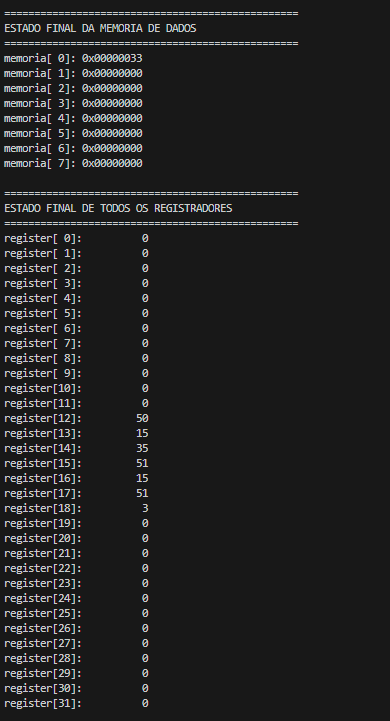
\includegraphics[width=0.4\textwidth]{teste.png}
    \caption{Estado final dos registradores e da memória de dados após execução do programa de teste.}
    \label{fig:resultado-simulacao}
\end{figure}

\subsection*{3.3. Análise da Execução de Instrução Aritmética (sub)}
\addcontentsline{toc}{subsection}{3.1. Análise da Execução de Instrução Aritmética (sub)}

O primeiro cenário de teste verifica a execução de uma instrução aritmética básica do Tipo-R, a \texttt{sub x14, x12, x13}. O objetivo é observar o caminho de dados desde a decodificação até a escrita do resultado no banco de registradores. A Figura \ref{fig:gtk_sub} exibe a forma de onda capturada durante a execução desta instrução.

\begin{figure}[H]
    \centering
    % --- COLOQUE O NOME DO SEU ARQUIVO DE IMAGEM AQUI ---
    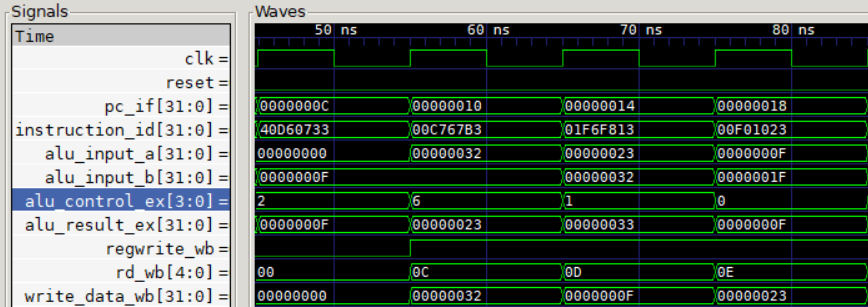
\includegraphics[width=1\textwidth]{Cenário 1.png}
    \caption{Forma de onda da execução da instrução \texttt{sub x14, x12, x13}.}
    \label{fig:gtk_sub}
\end{figure}

A análise da Figura \ref{fig:gtk_sub} revela o seguinte comportamento, ciclo a ciclo:
\begin{itemize}
    \item \textbf{Em 50ns:} A instrução \texttt{sub} (código \texttt{0x40D60733}) está no estágio de Decodificação (ID), como visto no sinal \texttt{instruction\_id}.
    
    \item \textbf{Em 60ns:} A instrução avança para o estágio de Execução (EX). Os sinais confirmam que a operação está correta:
    \begin{itemize}
        \item \texttt{alu\_input\_a} recebe o valor de x12, que é \texttt{0x32} (50).
        \item \texttt{alu\_input\_b} recebe o valor de x13, que é \texttt{0x0F} (15).
        \item \texttt{alu\_control\_ex} mostra o valor \texttt{6} (binário \texttt{0110}), que é o código correto para a operação de subtração.
        \item Como resultado, \texttt{alu\_result\_ex} exibe \texttt{0x23} (35), confirmando que a subtração (50 - 15) foi executada com sucesso.
    \end{itemize}
    
    \item \textbf{Em 80ns:} Após passar pelo estágio de Memória, a instrução chega ao estágio de Write Back (WB). Os sinais demonstram a conclusão da instrução:
    \begin{itemize}
        \item \texttt{regwrite\_wb} está em nível alto ('1'), habilitando a escrita no banco de registradores.
        \item \texttt{rd\_wb} indica o registrador de destino, que é \texttt{0E} (x14).
        \item \texttt{write\_data\_wb} contém o resultado final, \texttt{0x23} (35), que será escrito em x14.
    \end{itemize}
\end{itemize}

A análise da forma de onda valida com sucesso a execução de uma instrução do Tipo-R, confirmando que os estágios do pipeline, a unidade de controle e a ALU estão operando corretamente em conjunto.

\subsection*{3.4. Análise de Hazard de Dados com Forwarding}
\addcontentsline{toc}{subsection}{3.2. Análise de Hazard de Dados com Forwarding}

Este cenário testa uma das otimizações mais importantes do pipeline: a capacidade da Unidade de Forwarding de resolver um hazard de dados do tipo RAW (Read-After-Write) sem a necessidade de paralisar o processador. Analisamos a sequência de instruções \texttt{sub x14, x12, x13}, seguida imediatamente por \texttt{or x15, x14, x12}. A instrução \texttt{or} depende do resultado da \texttt{sub}, que ainda não foi escrito no banco de registradores.

A Figura \ref{fig:gtk_fwd} captura o momento exato em que a Unidade de Forwarding entra em ação.

\begin{figure}[H]
    \centering
    % --- COLOQUE O NOME DO SEU ARQUIVO DE IMAGEM AQUI ---
    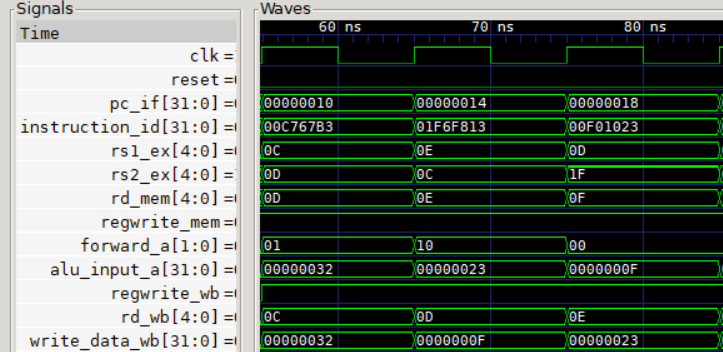
\includegraphics[width=1\textwidth]{Cenário2.png}
    \caption{Forma de onda demonstrando o forwarding do resultado de \texttt{sub} para \texttt{or}.}
    \label{fig:gtk_fwd}
\end{figure}

A análise da forma de onda, com foco no ciclo de clock entre 60ns e 70ns, revela:
\begin{itemize}
    \item \textbf{Condição de Hazard:} A instrução \texttt{or} está no estágio de Execução (EX) e precisa ler o registrador \texttt{x14} (o sinal \texttt{rs1\_ex} é \texttt{0E}). Ao mesmo tempo, a instrução anterior, \texttt{sub}, está no estágio de Memória (MEM) e seu registrador de destino é também o \texttt{x14} (\texttt{rd\_mem} é \texttt{0E} e \texttt{regwrite\_mem} está ativo).
    
    \item \textbf{Ação do Forwarding:} A Unidade de Forwarding detecta essa dependência e ativa o sinal de controle \texttt{forward\_a}, mudando seu valor para \texttt{10}. Este sinal instrui o MUX de entrada da ALU a ignorar o dado vindo do banco de registradores e, em vez disso, capturar o resultado que está saindo do estágio MEM.
    
    \item \textbf{Resultado:} O sinal \texttt{alu\_input\_a} mostra o valor \texttt{0x23} (35), que é o resultado da instrução \texttt{sub}. Isso confirma que o dado foi "adiantado" (forwarded) com sucesso do estágio MEM para o EX, permitindo que a instrução \texttt{or} execute sem atrasos e com o operando correto.
\end{itemize}

Este resultado valida o funcionamento da Unidade de Forwarding, uma otimização essencial para a eficiência de processadores com arquitetura pipeline.

\subsection*{3.5. Análise de Hazard de Controle com Flush}
\addcontentsline{toc}{subsection}{3.3. Análise de Hazard de Controle com Flush}

O último e mais complexo cenário de teste valida a resposta do processador a um hazard de controle. Analisamos a execução da instrução \texttt{beq x12, x12, +8}, um desvio que, por comparar um registrador com ele mesmo, será sempre tomado. Isso exige que o processador descarte as instruções que foram buscadas especulativamente, assumindo um fluxo sequencial.

A Figura \ref{fig:gtk_flush} captura o momento crítico em que a decisão do desvio é tomada no estágio MEM e o mecanismo de flush é acionado para corrigir o pipeline.

\begin{figure}[H]
    \centering
    % --- COLOQUE O NOME DO SEU ARQUIVO DE IMAGEM AQUI ---
    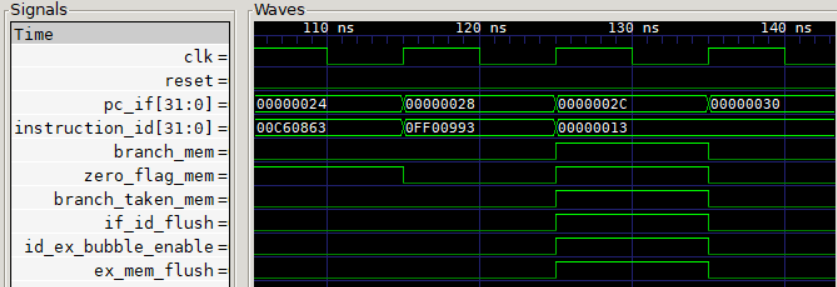
\includegraphics[width=1\textwidth]{Cenário 3.png}
    \caption{Forma de onda do flush no pipeline após um desvio condicional (\texttt{beq}) ser tomado.}
    \label{fig:gtk_flush}
\end{figure}

A análise da forma de onda, com foco no ciclo entre 110ns e 120ns, demonstra a sequência de eventos:
\begin{itemize}
    \item \textbf{O Gatilho (Estágio MEM):} A instrução \texttt{beq} está no estágio MEM. A sua condição é validada quando os sinais \texttt{branch\_mem} (indicando que é um desvio) e \texttt{zero\_flag\_mem} (indicando que o resultado da comparação foi zero) vão para nível alto. Como resultado direto, o sinal \textbf{\texttt{branch\_taken\_mem}} é ativado.

    \item \textbf{A Ação (Hazard Unit):} O sinal \texttt{branch\_taken\_mem} serve como entrada para a Unidade de Detecção de Hazards. Ela responde imediatamente ativando os três sinais de limpeza: \texttt{if\_id\_flush}, \texttt{id\_ex\_bubble\_enable} e \texttt{ex\_mem\_flush}.

    \item \textbf{A Consequência (Estágios IF e ID):} O efeito do flush é visível nos ciclos seguintes:
    \begin{itemize}
        \item No ciclo de 120ns, o \texttt{pc\_if} salta de seu valor sequencial (\texttt{0x24}) para o endereço de destino do desvio (\texttt{0x28}), corrigindo o fluxo do programa.
        \item No ciclo de 130ns, a instrução no estágio ID (\texttt{instruction\_id}) torna-se um NOP (\texttt{0x13}). Isso prova que a instrução incorreta (\texttt{addi x19,...}) foi com sucesso anulada e substituída por uma bolha.
    \end{itemize}
\end{itemize}

Esta simulação valida com sucesso o mecanismo de flush do pipeline, demonstrando que o processador consegue se recuperar de desvios tomados, garantindo a integridade da execução do programa.

% --- Seção de Referências ---
\begin{thebibliography}{9}
\addcontentsline{toc}{section}{Referências}

\bibitem{Patterson2017}
Patterson, D. A. and Hennessy, J. L. (2017). \textit{Computer Organization and Design RISC-V Edition: The Hardware Software Interface.} Morgan Kaufmann, Cambridge.

\end{thebibliography}

\end{document}